Segundo a Organização Mundial de Saúde (OMS) \cite{oms},
as doenças cardiovasculares são as principais
causas de óbitos no mundo. Cerca de 40\% dessas
mortes são ocasionadas por doenças na artéria
coronária (DAC). 

\medskip
Em 1964, Dotter e Judkins \cite{dotter1964} introduzem uma nova técnica para o tratamento
da artéria femoral obstruída devido a aterosclerose. Esta técnica é
conhecida como \textit{angioplastia transluminal percutânea} e consiste num
procedimento simples e minimamente invasivo, possibilitando a execução por qualquer 
médico familiarizado com a cateterização vascular. Tal procedimento se apresentou 
aplicável a outras artérias, inclusive a artéria coronária.

\medskip
Em 1979, Gruntzig, Senning e Seigenthaler \cite{gruntzig1979} realizam a técnica transluminal percutânea na artéria
coronária utilizando um cateter com balão inflável com o intuito de dilatar o local
com esterose. O procedimento foi realizado em 50 pacientes durante 18 meses e
apresentou-se resultados satisfatórios principalmente com pacientes com apenas
uma única artéria com esterose. Tal procedimento fica conhecido como \textit{Angioplastia Coronária
Transluminal Percutânea} (PTCA). 

\medskip
Embora o PTCA utilizando um balão inflável tenha apresentado resultados satisfatórios,
com o passar o tempo a artéria apresentava reestenose. Em 1987, Sigwart et al. \cite{sigwart1987}
apresentam o resultado da implantação de uma prótese constituida de uma malha de aço 
inoxidável auto-expansível nas artérias femoral e coronárias de 25 pacientes que apresentavam 
casos de reestenose. Embora a reestenose continuar presente, a prótese se mostrou uma
maneira interessante para a resolução da reestenose. Esta prótese recebeu o nome de \textit{stent}.

\medskip
Em 1994, Serruys et al. \cite{serruys1994} apresentam uma comparação entre os procedimentos PTCA 
utilizando um balão inflável e a implantação do stent. Foram analisados 520 pacientes,
onde 262 pacientes com stents implantados e 258 pacientes somente com o procedimento do
balão inflável. Os resultados clínicos e angiográficos apresentaram-se melhores para os
pacientes que tiveram a implantação do stent àqueles que fizeram o procedimento apenas
utilizando o balão inflável. Dessa forma, o procedimento PTCA com a implantação do stent
foi confirmado como uma solução mais eficaz que o PTCA utilizando apenas o balão inflável. 
Porém, um problema persistia: a reestenose. Ao decorrer da década de 90, os pesquisadores 
buscavam resolver este problema. A \ref{procedimentos PTCA} apresenta o comparativo entre
os procedimentos PTCA com o uso do balão inflável e do stent.

\begin{figure}[H]
     \begin{minipage}{.50\linewidth}
      \centering
      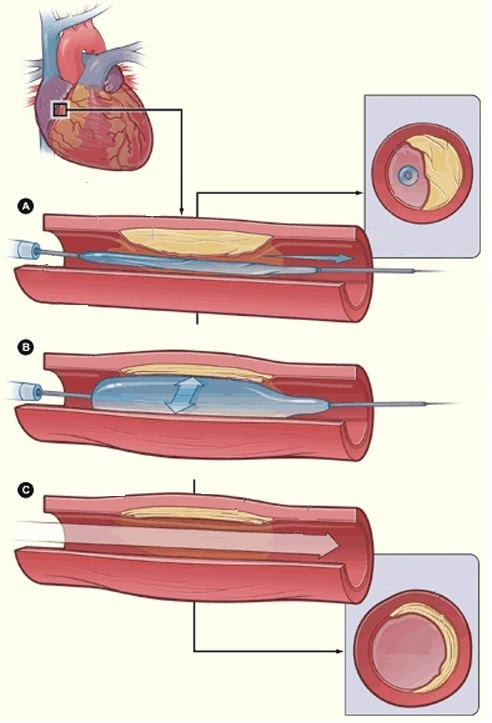
\includegraphics[scale=0.5]{./02_chaps/cap_review/figure/balloon.jpg}\\
      (a)
     \end{minipage}%
     \begin{minipage}{.50\linewidth}
      \centering
      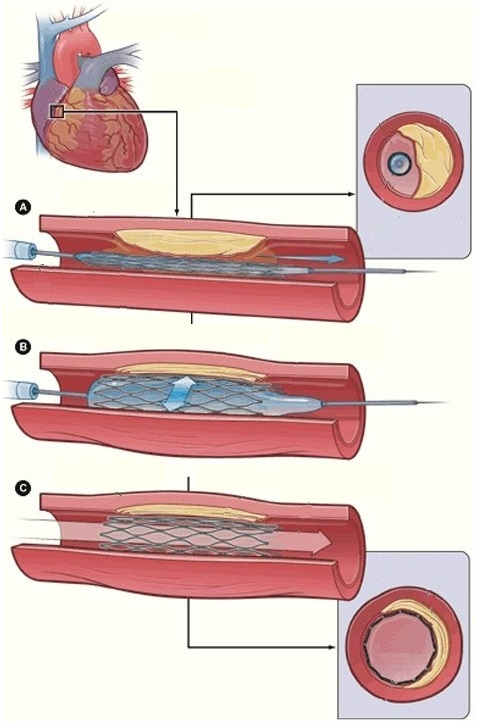
\includegraphics[scale=0.5]{./02_chaps/cap_review/figure/stent_bare.jpg}\\
      (b)
     \end{minipage}
     \medskip
     \caption{Comparativo dos procedimentos PTCA:
              (a) balão inflável e
              (b) stent.}
     \label{procedimentos PTCA}
\end{figure}

\medskip
Em 2001, Hwang, Wu e Edelman \cite{hwang2001} apresentam uma simulação da implantação de um stent
revestido com uma droga em uma artéria coronária. A simulação apresentou a 
intima relação entre a distribuição da droga e o \textit{número de Peclet} 
além da importância em desenvolver geometrias para os stents que potencializem 
a difusão da substância química. Tal procedimento se mostrou uma opção promissora
para o tratamento da aterosclerose e da reestonose. Este novo tipo de stent
ficaria conhecido como \textit{stent farmacológico}.

\medskip
Em 2014, Bozsak, Chomaz e Barakat \cite{bozsak2014} propõem um modelo computacional de transporte
das drogas \textit{paclitaxel} e \textit{sirolimus} na parede da artéria. Tais drogas são 
frequentemente usadas em stents farmacológicos. O modelo leva em conta a estrutura em
multicamadas da parede da artéria e essas camadas foram modeladas como meios porosos.
Desta forma, a lei de \textit{Darcy} foi utilizada para simular o escoamento dentro das camadas
da artéria. A simulação apresentou que a escolha do tipo de droga utilizada
é um paramêtro crucial na criação do stent farmacológico
devido ao transporte na parede da artéria. 

\medskip
Recentemente, Lucena et al. \cite{lucena2017} apresentam
a simulação do transporte da droga \textit{sirolimus} na parede de uma artéria modelada
como um meio poroso e anisotrópico. Foi considerado a dissolução no revestimento polimérico
do stent além do transporte na parede da artéria em um domínio axissimétrico. As equações
de governo foram aproximadas segundo o Método dos Elementos Finitos. O trabalho apresentou
que o tempo de evolução do processo de transporte pode ser eficientemente controlado 
pelo coeficiente de difusão do polímero. É estimado que cerca de 47\% da droga é difundida
no lúmen sendo perdida na corrente sanguínea. A distruibuição espacial da droga, porém, é
grandemente influenciada pelo escoamento sanguíneo e as propriedades da parede da artéria.
Assim, tais resultados são suscetíveis às condições de saúde do paciente.

\medskip
No mesmo ano, Wang et al. \cite{wang2017} apresentam a simulação do escoamento sanguíneo
em uma artéria coronária com aterosclerose e stent farmacológico implantado. O sangue
é aproximado como um fluido newtoniano e monofásico e as equações de governo segundo as 
variáveis primitivas foram aproximadas segundo o Método dos Elementos Finitos. 
Foram apresentadas diversas geometrias axissimétricas inclusive uma artéria coronária real. 
Tais geometrias foram aproveitadas para
este atual trabalho, porém modificadas para uma abordagem bidimensional. As simulações 
apresentaram que o modelo simplificado da artéria com aterosclerose proposto produzia resultados
semelhantes de velocidade, pressão e concentração quando comparados com a artéria real.

\medskip
Ao longo da década passada e atual, diversos stents farmacológico foram desenvolvidos tais como:
\textit{Ravel} \cite{morice2002}, 
\textit{Taxus I e Taxus II} \cite{grube2003} \cite{colombo2003}, 
\textit{C-Sirius} \cite{schampaert2004}, 
\textit{Smart} \cite{ardissino2004} e outros mais recentes como
apresentado na \ref{stent drug}. Atualmente, uma nova geração
de stents tem sido desenvolvida em que toda a estrutura é 
absorvida. Tal geração é conhecida como \textit{stent bioabsorvível},
o uso desta tecnologia não é assunto deste trabalho.

\begin{figure}[H]
  \centering
  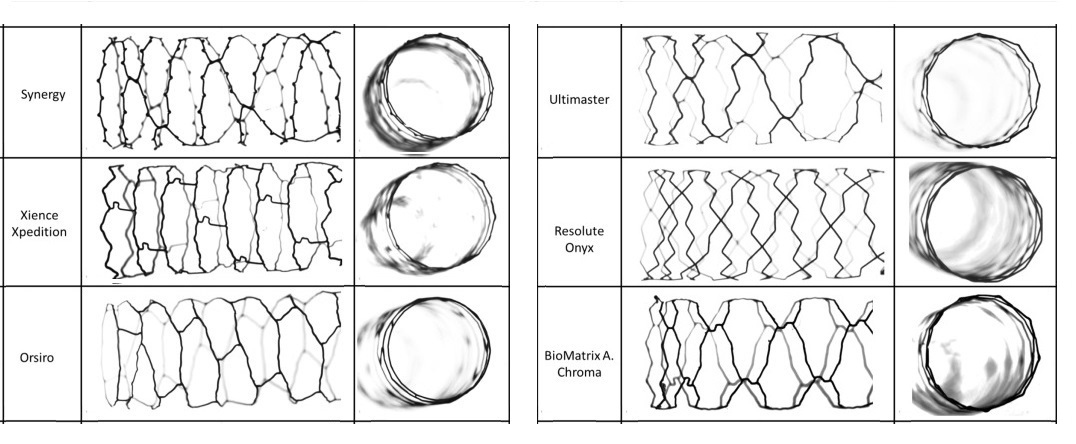
\includegraphics[scale=0.66]{./02_chaps/cap_review/figure/stent_drug.jpg}
 \caption{Diversos modelos de stent farmacológico \cite{stent2016}.}
 \label{stent drug}
\end{figure}

